

For evaluating our approach, we collect a dataset of videos using an iPhone X, with a stationary subject and the camera moving from one profile to the other. The videos are shot at the 120fps setting and are typically 15-20 seconds long, depending on whether they are shot by the subject themselves or by an assistant. The background conditions are unconstrained, though we do ensure a mostly static scene to get accurate camera pose estimates from our Photometric Bundle Adjustment step.

%%%%%%%%%%%%%%%%%%%%%%%%%%%%%%%%%%%%%%%%%%%%%%%%%%%%%%%%%%%%%%%%%%%%%%%%%%%%%%55
%%%%%%%%%%%%%%%%%%%%%%%%%%%%%%%%%%%%%%%%%%%%%%%%%%%%%%%%%%%%%%%%%%%%%%%%%%%%%%%%5
\section{Quantitative Evaluation} \label{sec:quant}

For 10 subjects among the videos we collected, we obtained high accuracy 3D face scans using an Arctic Eva structured light hand-held scanner. The scans were obtained immediately after the video was recorded with the subjects still in the same poses, to ensure no discrepancy in face geometry between the video and the scan. We use the videos of these subjects to reconstruct face meshes using the methods listed in Table \ref{table:results}. For methods that work on a single image, we use a close to frontal keyframe as input. For the edge-fitting based single view method of Bas \etal \cite{bas2016fitting}, we select a frame at roughly 15 degrees to the front for the input, since that was reported to work best in their paper. For the multi-view methods, we either use the keyframes generated by our method or the whole video, depending on what the method uses as input.
% However the methods of Roth \etal and PCSfM are not able to make use of all of our keyframes as they are reliant on landmark detectors for alignment and pose estimation, and so typically only use frames in a cone around the front of the face. For the method of multi-view landmark fitting, we use the whole video, using the implementation provided in 4dface \cite{huber2016multiresolution}). 
For all methods except PCSfM, the authors make their implementations public and we use those for evaluation. For PCSfM, we use our own implementation.

A challenge in fair quantitative evaluation arises from the fact that different methods reconstruct different amounts of the face area as defined by the Basel mesh, such as frontal only in pix2vertex \cite{sela2017unrestricted} , front and side without ears in PRN \cite{feng2018joint}, full Basel mesh for PCSfM \cite{hernandez2017accurate} and arbitrary in SfM (using COLMAP \cite{schonberger2016structure}). To address this, we first register a standard Basel mesh to the ground truth 3D scans using Non-rigid ICP \cite{amberg2007optimal,booth2018large}. We then borrow a strategy from MVS benchmarks \cite{jensen2014large,knapitsch2017tanks,yao2018mvsnet} to evaluate the reconstructions using \textbf{Accuracy} - the distance from the reconstruction's vertices to the ground truth, and \textbf{Completion} - the distance from the ground truth's vertices to the reconstruction. Thus, if a method reconstructs only the frontal face, it might do well in Accuracy and be penalized in Completion. We report the mean and median of these distances, averaged over the 10 subjects, in Table \ref{table:results}.

We compare our methods against several recent single and multi-view reconstruction methods. 
As can be observed, single view methods typically have very poor performance in terms of accuracy and completion. 
As also noted in \cite{hernandez2017accurate}, certain methods that just reconstruct smooth meshes tend to have low numeric errors, even if the reconstruction lacks details important for making a person recognizable.

Our method clearly outperforms single and multi-view baselines, both in terms of accuracy and completion. We note that our median accuracy is around 0.95 mm, showing that for majority of the mesh we achieve sub-millimeter accuracy.

\subsection{Ablation} We generate reconstructions without Edge constraints and without the ear landmarks respectively. Edges improve the accuracy of the reconstructions by improving the fit of areas like the jaw and nose, whereas the ear landmarks improve the information captured in the ears as well as overall mesh scale and width. Thus dropping either leads to a drop in accuracy. A significant drop in completion is also observed when removing the ear landmarking, because the reconstructed mesh moves away from the ears of the ground truth mesh.




\begin{table}
\begin{center}
\begin{tabular}{|c|c|c c c|c c c|}
\hline 
\multirow{2}{*}{Method} & \multirow{2}{*}{Views} 
& \multicolumn{3}{c|}{Accuracy (mm) $\downarrow$} 
& \multicolumn{3}{|c|}{Completion(mm) $\downarrow$} \\ 
\cline{3-8}
& & Mean & Std. Dev. & Median & Mean & Std. Dev. & Median\\
\hline\hline
Mean Basel \cite{blanz1999morphable}       & - & 3.09  & 1.24 &  2.62 & 3.02 & 1.25  & 2.76 \\ 
Landmark fitting \cite{huber2016multiresolution}  & Single  & 2.53  & 0.62 & 1.88 & 8.01     & 2.13 & 3.62      \\ 
pix2vertex \cite{sela2017unrestricted} & Single & 3.49 & 0.76 & 2.76 & 25.33 & 4.62 & 16.34  \\
PRN \cite{feng2018joint} & Single & 2.63 & 0.84 & 2.30 & 6.27 & 2.17 & 3.24 \\
Edge-fitting \cite{bas2016fitting} & Single & 3.06 & 1.28 & 2.63 & 3.02 & 1.25 & 2.75 \\

\hline
M.view lm fit \cite{huber2016multiresolution,huber2015fitting} & Multi   & 2.23 & 0.41 &    1.69   & 7.87          & 1.98 & 3.59   \\ 
Roth \etal \cite{roth2015unconstrained}     & Multi   & 3.31 & 1.03 & 2.65 & 7.65 & 1.86 & 3.67 \\
SfM \cite{schonberger2016structure} & Multi & 5.42 & 2.55 & 3.61 & 4.72 & 2.41 & 3.60 \\
PCSfM* \cite{hernandez2017accurate} & Multi & 1.87 & 0.40 & 1.66 & 2.38 & 0.85 & 2.04 \\
\hline
Ours w/o Edges    &  Multi  & 1.38 & 0.24 & 0.98 & 1.30 & 0.29 & 0.97 \\
Ours w/o ear lms    &  Multi     & 1.33 & 0.27 & 0.96 & 1.41 & 0.36& 1.07      \\
Ours    &  Multi     & \textbf{1.24} & 0.26 & \textbf{0.95} & \textbf{1.29} & 0.29 & \textbf{0.95}     \\

% \specialrule{.16em}{.08em}{.081em}
\hline
\end{tabular}
\end{center}
\caption{Quantitative results against ground truth scans. We evaluate the state of the art single and multi-view reconstruction methods. As is common in MVS benchmarks, we evaluate the reconstructions in terms of average distance from reconstruction to ground truth (accuracy) and distance from ground truth to reconstruction (completion). All numbers in mm; lower is better. * denotes that the method needs camera intrinsics to be known in advance.}
\label{table:results}
\end{table}


\begin{figure*}
\begin{center}
   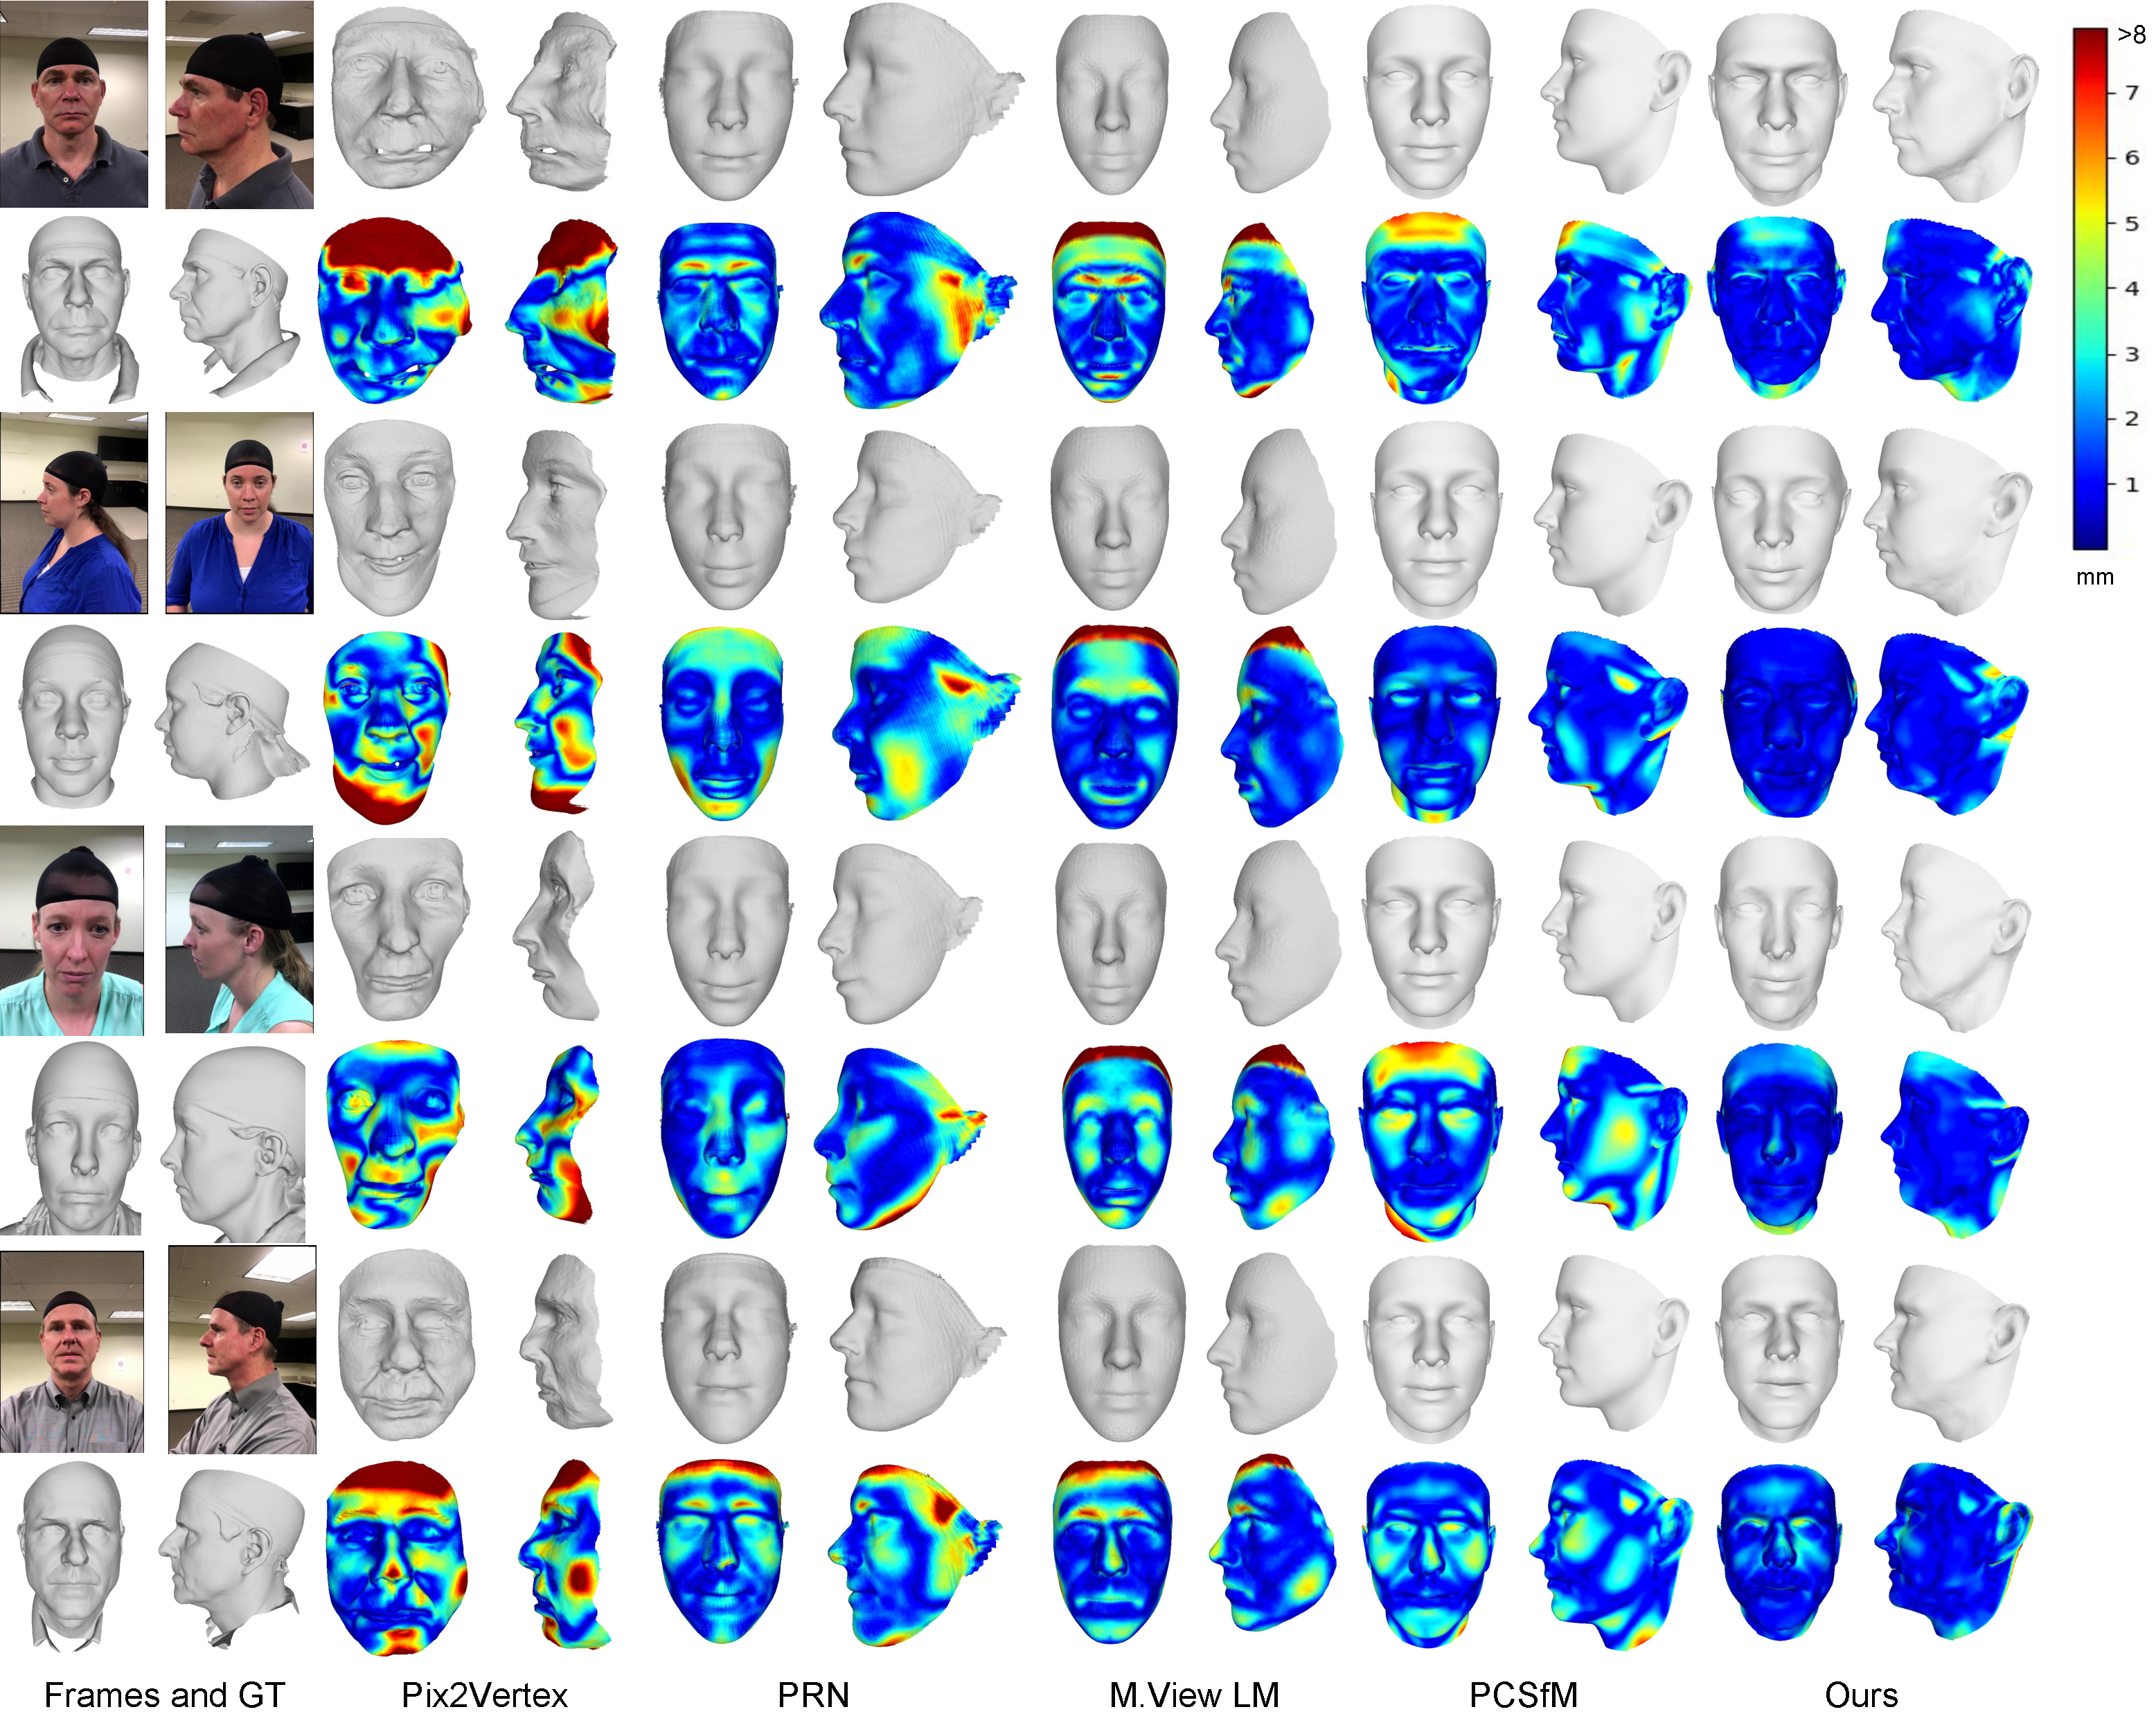
\includegraphics[width=1\linewidth]{images/qual_figure.pdf}
\end{center}
  \caption{Qualitative comparison against reconstructions of various single and multi-view methods. Let to Right: sample frame and ground truth 3D, Pix2vertex \cite{sela2017unrestricted}, PRN \cite{feng2018joint}, multi-view landmark fitting (4dface \cite{huber2016multiresolution}), PCSfM \cite{hernandez2017accurate}, Ours. For each method the upper row shows the reconstructed mesh, front and profile, and the corresponding heatmap of error (Accuracy) is shown in the lower row }
\label{fig:results}
\end{figure*}


\begin{figure}
\begin{center}
% \fbox{\rule{0pt}{2in} \rule{0.9\linewidth}{0pt}}
   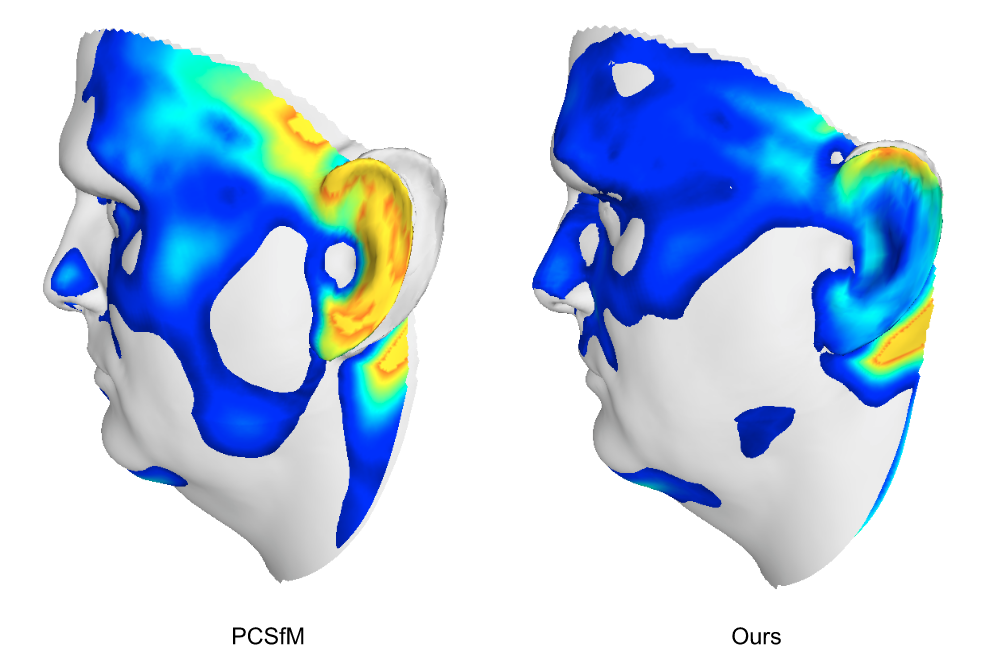
\includegraphics[width=0.8\linewidth]{images/ear_align.png}
\end{center}
   \caption{Effect of ear landmarking: Ground truth mesh (white) overlapped with error heatmaps of PCSfM(left) and ours(right). Landmarking the ears greatly improves our fitting and reduces the geometric error in our reconstructions }
\label{fig:ear_align}
\end{figure}

\begin{figure}
\begin{center}
% \fbox{\rule{0pt}{2in} \rule{0.9\linewidth}{0pt}}
   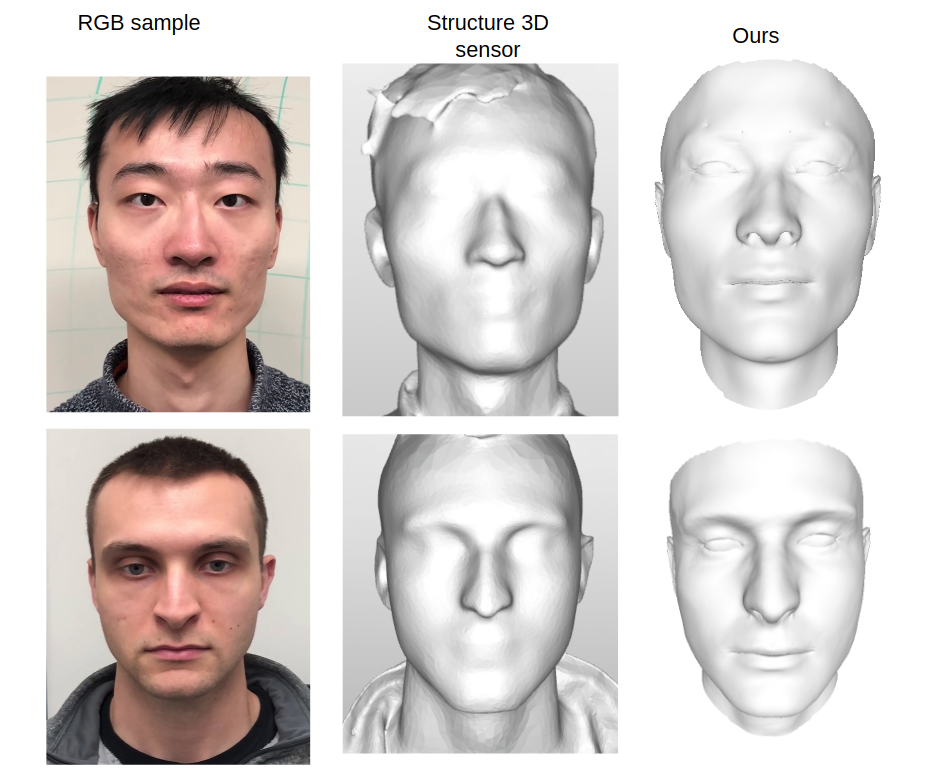
\includegraphics[width=0.8\linewidth]{images/struc_3d_comp.png}
\end{center}
   \caption{(Middle) Output from Structure RGB-D Sensor \cite{structure2019}. Details like the eyes, nose and lips are excessively smoothed out. (Right) Our reconstruction.}
\label{fig:long}
\label{fig:onecol}
\end{figure}





\section{Expressions}

Our method captures the geometry of the face in a completely data-driven manner, and hence it also generalizes naturally to deformations caused by expressions (Fig \ref{fig:exp}). Since, is difficult to hold the same expression through a video sequence and then also obtain a corresponding ground truth 3D scan, we skip quantitative evaluation of this. 
We also note that since there is dense correspondence and consistent topology across meshes, various existing techniques like blendshapes \cite{cao2014facewarehouse}  can be applied with our reconstructed meshes to generate animated, expressive face models.


\begin{figure}[t]
\begin{center}
   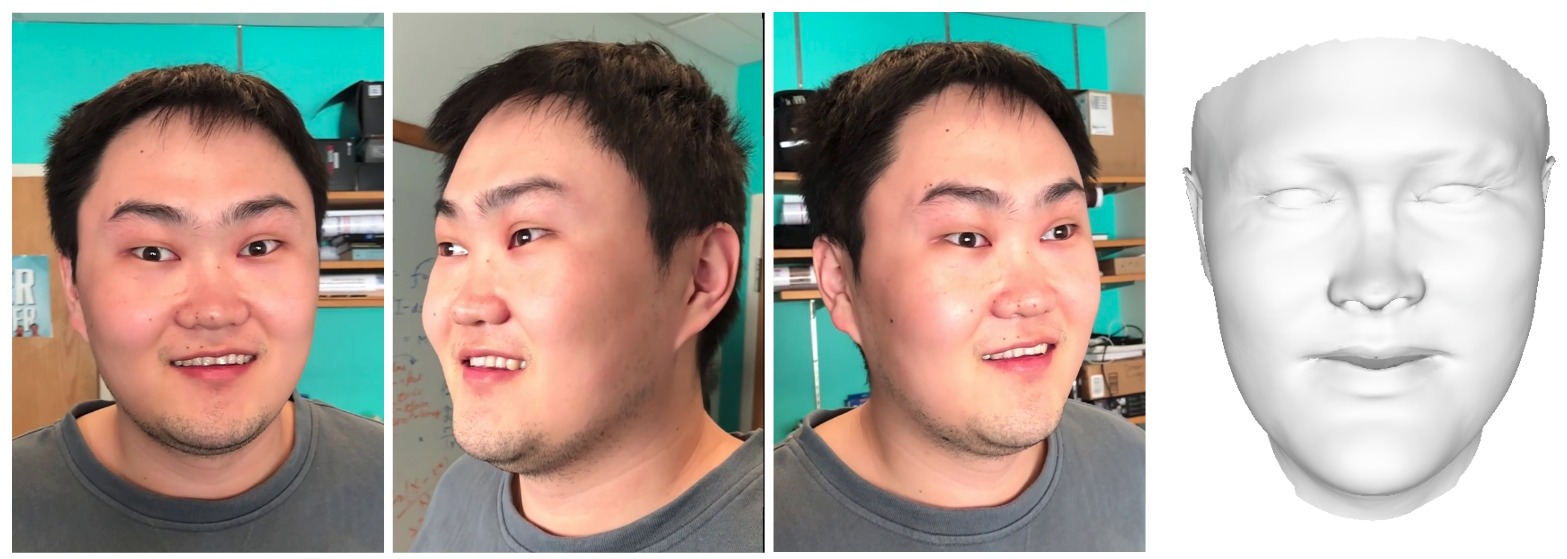
\includegraphics[width=0.9\linewidth]{images/expressions.png}
\end{center}
   \caption{Our method naturally generalizes to any face geometry, including deformations caused by expressions. }
\label{fig:exp}
\end{figure}